\documentclass[9pt,aspectratio=169]{beamer}

\usepackage{nicefrac}

\usetheme{graham}

\title{Geometric sequencies}
\subtitle[Graham Middle School]{Graham Middle School Math Olympiad Team}

\begin{document}
\maketitle

\begin{frame}{Geometric series and the invention of chess}
  \begin{columns}[T]
    \begin{column}{0.5\textwidth}
      This story happened (\emph{or probably not}) in the Persian Empire (\emph{or probably in India}).  The Shah (king) was so delighted by the game of chess that he invited its creator to his court and asked him to make any wish as a reward for creating the game.  

      The clever inventor said, “Oh generous Shah, all I ask is that you place $1$ grain of rice (\emph{or probably wheat}) on the first square, $2$ grains on the second square, $4$ grains on the 3\textsuperscript{rd} square, and continue doubling until you reach the 64\textsuperscript{th} square.”
      \begin{wrapfigure}{r}{0.32\textwidth}
        \vspace*{-1.5em}
        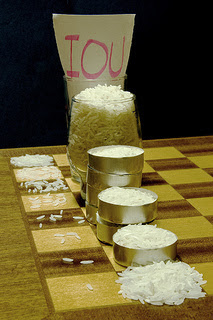
\includegraphics[width=0.35\textwidth]{07 - Geometric Sequences/rice.jpg}
      \end{wrapfigure}
      “Is that all you ask for?” laughed the Shah.  “I would have happily given you a fortune in gold.  But if that is your request, I promise you shall have it.”  With this promise made, an imperceptible grin spread over the inventor’s face as he bowed and took his leave of the Shah. 
    \end{column}
    \begin{column}{0.5\textwidth}
      The court mathematician was in attendance and overhead this conversation.  “Oh, powerful Shah,” began the alarmed mathematician, “we cannot meet his request.  It would bankrupt the kingdom.”  After the Shah heard the explanation, he summoned his guards to bring him the inventor and had him beheaded for his insolence (\emph{or hire him as a minister}).  How many grains of rice would have been required to satisfy the request?

      \begin{example}
        This request was asking the king to sum the terms of a geometric series
        \[ 1 + 2 + 4 + 8 + \ldots + 2^{63}. \]
        The total amount of grains was
        \[ 2^{64} - 1 = 18{,}446{,}744{,}073{,}709{,}551{,}615 \]which is enough to feed \emph{100 tons} of rice to every single human on Planet Earth.
      \end{example}
    \end{column}
  \end{columns}
\end{frame}

\begin{frame}{Geometric sequences}
  \begin{columns}[T]
    \begin{column}{0.5\textwidth}
      \emph{Binary fission} is the process by which bacterium divide into two identical daughter cells.

      \begin{problem}
        After $3$ minutes of life, a bacterium divides into two new bacteria. A new bacterium also split into two bacteria after $3$ minutes, and so on. One bacterium gets into a cup with a nutrient solution. How many bacteria will be in a cup after one hour?
      \end{problem}

      After $3$ minutes, it would be $2$ bacteria. After $6$~minutes, it would be $4$ bacteria and so on. Every $3$~minutes amount of bacteria doubled. Since an hour contains $20$ $3$ minutes intervals, the number of bacteria will be doubled $20$ times. So total amount of bacteria after one hour would be 
      \[ 1 \times 2^{20} = 1{,}048{,}576 \approx 1 \text{ million bacteria.} \]
      The sequence $1$, $2$, $4$, $8$, $\ldots$, $2^{20}$ is called a~geometric sequence.
    \end{column}
    \begin{column}{0.5\textwidth}
      \begin{definition}
        A \textbf{geometric sequence} is a sequence of numbers in which the ratio between \emph{consecutive terms} is the same.
        
        The \emph{ratio} between consecutive terms is called the \textbf{common ratio} of the sequence. 
      \end{definition}
      The common ratio is usually denoted as $r$.

      Some examples
      \[
        \begin{array}{l r r}
          \text{geometric sequence}\hspace*{3em} & a_1 & \hspace*{2em}r \\
          1,\ 2,\ 4,\ 8,\ 16,\ 32,\ \ldots & 1 & 2 \\[0.4em]
          3,\ 1,\ \dfrac{1}{3},\ \dfrac{1}{9},\ \dfrac{1}{27},\ \ldots & 3 & \dfrac{1}{3} \\[0.7em]
          1,\ -1,\ 1,\ -1,\ 1,\ -1,\ 1,\ \ldots & 1 & -1 \\
          2,\ 2,\ 2,\ 2,\ 2,\ \ldots & 2 & 1
        \end{array}
      \]
      A sequence can also have \emph{infinitely} many terms.

      \begin{definition}
        A general term ($n$\textsuperscript{th} term) of a geometric sequence may be found using formula
        \[ a^n = a_1 × r^{n-1}. \]
        \vspace*{-1\baselineskip}
      \end{definition}
    \end{column}
  \end{columns}
\end{frame}

\begin{frame}{Geometric series}
  \begin{columns}[T]
    \begin{column}{0.5\textwidth}
      \begin{definition}
        The \emph{sum} of the terms of a geometric sequence is called a \textbf{geometric series}.
      \end{definition}
      \begin{problem}
        Find the sum $1 + 3 + 9 + 27 + 81 + 243 + 729$.
      \end{problem}

      Direct summation gives us $1093$. But what to do if series would be longer?

      Let’s multiply this sum (denoted as $S$) by the common ratio
      \[ 3S = 3 + 9 + 27 + 81 + 243 + 729 + 2187. \]
      It looks exactly the same as the original sum except $1$ has been replaced with $2187$.  So 
      \[ 3S = S - 1 + 2187. \]
      Solving for $S$
      \[ S = \frac{2187 - 1}{3 - 1} = \frac{2186}{2} = 1093. \]
    \end{column}
    \begin{column}{0.5\textwidth}
      Let’s get general formula for a geometric series.
      
      The initial term is $a$, the ratio is $r$, and we have a~total of $n$ terms. Hence we have the following series
      \[ S = a + a \times r + a \times r^2 + \ldots + a \times r^{n-1}. \]Multiply it by $r$
      \[ S \times r = a \times r + a \times r^2 + \ldots + a \times r^{n-1} + a \times r^n. \]
      Subtract the initial sum
      \[ S \times r - S = a \times r^n - a. \]
      \vspace*{-1em}
      \begin{definition}
        The sum of geometric sequence is
        \[ S = \frac{a \times r^n - a}{r - 1}\]
        \vspace*{-0.7em}
      \end{definition}
      Note, if $r = 2$, the formula become $S = a \times 2^n - a$, which gives us the total amount of grains the Shah owes to the inventor of chess.
    \end{column}
  \end{columns}
\end{frame}

\begin{frame}{Infinite geometric series}
  \begin{columns}[T]
    \begin{column}{0.5\textwidth}
      The series goes on forever in an infinite geometric series, with a constant ratio between successive terms.  What is the sum of the elements of an infinite geometric series?

      If $r \geq 1$, the sum is infinite since we have an infinite number of non-zero terms that are either staying constant ($r = 1$) or growing ($r > 1$).
      
      If $r < 1$, however, the series is said to \emph{converge}. It is possible to calculate the value of the sum of the elements in the series.

      \begin{problem}
        Find the sum $\dfrac{1}{2} + \dfrac{1}{4} + \dfrac{1}{8} + \dfrac{1}{16} + \dfrac{1}{32} + \ldots$. 
      \end{problem}

      Let $S$ is the sum of the elements in the series.
      
      $S = \nicefrac{1}{2} + \nicefrac{1}{4} + \ldots$ Now multiply both sides of the equation by $2$.
      
      $2S = 1 + \nicefrac{1}{2} + \nicefrac{1}{4} + \ldots$ Wait, isn’t the right side of the equation just $1 + S$?
      
      So $2S = 1 + S$ (now subtract $S$ from both sides)
      
      $S = 1$.  So, the sum of $\nicefrac{1}{2} + \nicefrac{1}{4} + \ldots = 1$.

    \end{column}
    \begin{column}{0.5\textwidth}
      \begin{wrapfigure}[11]{r}{0.4\textwidth}
        \vspace*{-1.5em}
        \hspace*{-2em}
        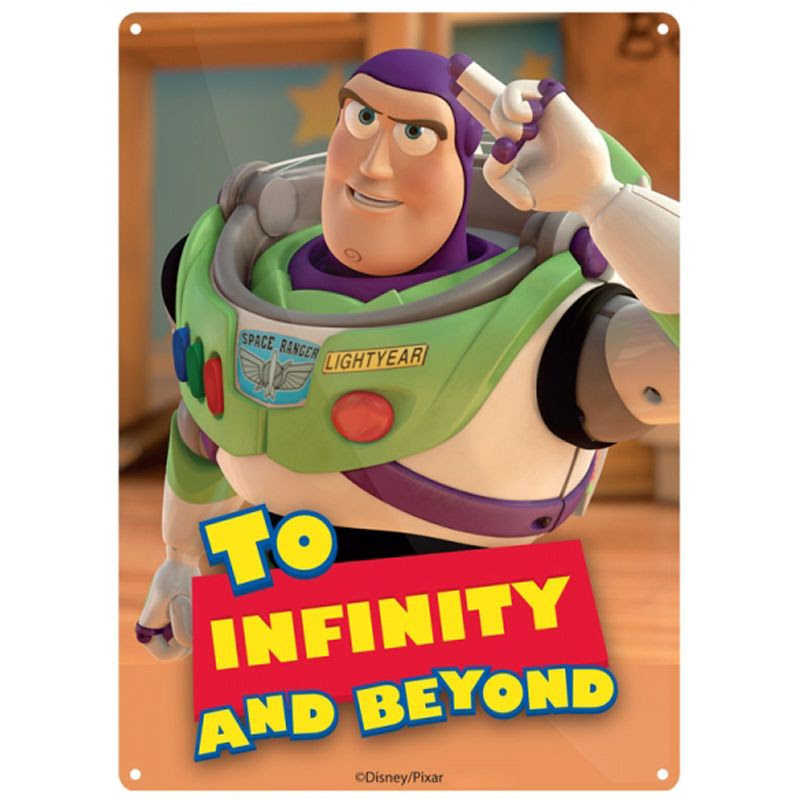
\includegraphics[width=0.6\textwidth]{07 - Geometric Sequences/infinity.jpg}
      \end{wrapfigure}
      For positive numbers $r < 1$, as $n$ becomes arbitrarily large, $r^n$ \emph{tends to zero}. And, taking the \emph{limit of the sequence}, we can consider $r^n$ is equal to $0$ when $n$ goes to infinity.
      
      Let’s apply this to the formula for the sum of a~geometric sequence when $-1 < r < 1$ and for infinite sequence.
      \[ S = \frac{a \times r^n - a}{r - 1} = \frac{-a}{r - 1} = \frac{a}{1 - r}. \]
      \begin{definition}
        The sum of an infinite geometric series with a~common ratio less than $1$ 
        \[ S = \frac{a}{1 - r}. \]
        \vspace*{-0.5em}
      \end{definition}
    \end{column}
  \end{columns}
\end{frame}

\begin{frame}{Achilles and the tortoise}
  \begin{columns}[T]
    \begin{column}{0.5\textwidth}
      \emph{Zeno of Elea} was a Greek philosopher born around 490 BC.  He wrote a book featuring 40 paradoxes, of which \emph{Achilles and the Tortoise} is perhaps the most famous.
      
      Achilles, the ancient Greek hero, is chasing after a tortoise. Achilles is much faster than the tortoise, and so he must eventually catch up with it. 
      
      Zeno argued that on his way to catching the tortoise, Achilles must first reach the tortoise’s starting point. By the time he has reached this however, the tortoise will also have moved further forward to a new point. 
      \begin{wrapfigure}[7]{r}{0.32\textwidth}
        \vspace*{-2em}
        \hspace*{-1.3em}
        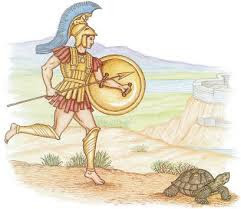
\includegraphics[width=0.45\textwidth]{07 - Geometric Sequences/zeno.jpg}
      \end{wrapfigure}
      By the time Achilles reaches this new point, the tortoise will have moved a bit further forward and so on. Every time Achilles reaches the point where the tortoise was, the tortoise has moved forwards to a new point. Hence Achilles \textbf{will never catch up}.
    \end{column}
    \begin{column}{0.5\textwidth}
      Let’s say Achilles run $10$ \emph{meters per second} and the tortoise’s speed is $0.1$ \emph{meters per second} and initial distance between them was $100$ meters. After $10$ seconds Achilles run $100$ meters and the tortoise crawled only $1$ meters. The next $0.1$ seconds Achilles run $1$ meter and the tortoise crawled $0.01$ meters and so on. 
      
      The distance and time will form infinite geometric series:
      
      Distance (m): $100 + 1 + 0.01 + 0.0001 + \ldots$
      
      Time (s): $10 + 0.1 + 0.001 + 0.00001 + \ldots$
      
      Let’s find the sums
      \begin{align*}
        \text{distance} &= \frac{100}{1 - 0.01} = \frac{100}{0.99} \approx 101.0101 \text{ m}, \\
        \text{time} &= \frac{10}{1 - 0.01} = \frac{10}{0.99} \approx 10.101 \text{ s}.
      \end{align*}
      As we see, “never” will happen $10.1$ seconds after the race begins, and Achilles catches the tortoise almost immediately when he gets to its starting point.
    \end{column}
  \end{columns}
\end{frame}

\begin{frame}{Repeating decimal}
  \begin{columns}[T]
    \begin{column}{0.5\textwidth}
      We instantly recognize the fractional representations for some repeating decimals.  For example, $0.333\ldots = \dfrac{1}{3}$ , $0.111\ldots = \dfrac{1}{9}$.  
      
      A repeating decimal can be represented as an infinite geometric series, and the sum of that series can be used to calculate the fractional representation for that repeating decimal.
      \begin{problem}
        Represent $0{.}4444\ldots$ as a common fraction.
      \end{problem}
      This is the sum of the infinite geometric series 
      \[0.4 + 0.4 \times 0.1 + 0.4 \times 0.1^2 + 0.4 \times 0.1^3 + \ldots \]\vspace*{-1\baselineskip}
      \begin{align*}
        S &= 0.4 + 0.4 \times 0.1 + 0.4 × 0.1^2 + \ldots \\
        10 \times S &= 4 + 0.4 + 0.4 × 0.1 + 0.4 × 0.1^2 + \ldots \\
        10 \times S &= 4 + S \\
        9 \times S &= 4 \\
        S &= \frac{4}{9}.
      \end{align*}
    \end{column}
    \begin{column}{0.5\textwidth}
      \begin{problem}
        What if there is more than one repeating digit in the decimal, such as $0.81818181\ldots$?  
      \end{problem}
      We can once again represent this as the sum of a~geometric series, but now the $r$ is $0.01$.
      \begin{align*}
        S &= 0.81 + 0.81 \times 0.01 + 0.81 \times 0.01^2 + \ldots \\
        100 \times S &= 81 + 0.81 + 0.81 \times 0.01 + \ldots \\
        100 \times S &= 81 + S \\
        99 \times S &= 81 \\
        S &= \frac{81}{99}.   
      \end{align*}
      In general every repeating decimal fraction with period of length $n$ may be represented as a~common fraction
      \begin{definition}
        \vspace*{-0.4em}
        \[ 0.a_1 a_2\ldots a_n a_1 \ldots = \frac{0.a_1 a_2\ldots a_n}{1 - 0.\underbrace{0\ldots0}_\text{$n$ times}1} = \frac{a_1 a_2\ldots a_n}{\underbrace{999\ldots 9}_\text{$n$ times}}. \]
        \vspace*{-0.4em}
      \end{definition}
    \end{column}
  \end{columns}
\end{frame}

\begin{frame}{Exercises}
  \begin{columns}[T]
    \begin{column}{0.5\textwidth}
      \begin{enumerate}
        \item Find the third term of the geometric sequence $2$, $3$, $\ldots$
        \item The first term of a geometric sequence is $1$, the third term is $4$. Find the second term. Is your answer the only possible one?
        \item Express the repeating decimal $0.636363\ldots$ as a fraction.
        \item Express the repeating decimal $0.9428571428571428\ldots$ as a fraction.
        \item For what value of $x$ does the infinite geometric series $1 + x + x^2 + x^3 + \ldots = 4$?
        \item If we subtract the geometric series $1 + \dfrac{1}{4} + \dfrac{1}{16} + \ldots$ from the infinite geometric series $1 + \dfrac{1}{2} + \dfrac{1}{4} + \ldots$, what is the sum of the resulting infinite geometric series?
        \seti
      \end{enumerate}
    \end{column}
    \begin{column}{0.5\textwidth}
      \begin{enumerate}
        \conti
        \item Find a digit $d$, so $0.d25d25d25\ldots = \dfrac{n}{810}$ for some positive integer $n$.
        \item Find a geometric sequence in which $8$, $18$, and $27$ are terms (not necessary adjacent).
      \end{enumerate}
    \end{column}
  \end{columns}
\end{frame}

\begin{frame}{Challenge problems}
  \begin{columns}[T]
    \begin{column}{0.5\textwidth}
      \begin{enumerate}
        \item Consider the alternating geometric series 
        $1 - \dfrac{1}{2} + \dfrac{1}{4} - \ldots.$   What is the sum of all of the positive terms in the series?  What is the sum of all of the negative terms in the series?  Show that when you add these two sums together, the sum of the entire series agrees with the formula for an infinite geometric series whose first term is $1$, with a value of $r = -\dfrac{1}{2}$.
        \item Let $N$ be defined as the infinite series of square roots shown below.  What is the value of $N$?
        \[ N = \sqrt{2021 \sqrt{2021 \sqrt{2021 \sqrt{\ldots}}}}\]
        \item Find the way to represent a fraction started  $0.010204081632\ldots$ with just $4$ symbols.
        \seti
      \end{enumerate}
    \end{column}
    \begin{column}{0.5\textwidth}
      \begin{enumerate}
        \conti
        \item A pirate captures $4$ math Olympiad team members named Alex, Beth, Colette, and Daniel.  He hands them a standard pair of $6$-sided dice and says, “I am going to have some fun with you.  You will take turns rolling the dice in alphabetical order (A, B, C, D, A, B, C, D, A, ..), and keep rolling until one of you rolls the dice so they sum to $7$. 
        I will set the first kid to roll a $7$ free and execute the rest, unless you can tell me what the probability of Daniel winning the game is, in which case I will let you all go.”  What is the answer to the pirate’s question (what is the probability that the last of the $4$ players to roll will win this game)?  Would Daniel’s odds of winning go up or down if players needed to roll double $6$’s instead of $7$ to win the game?
      \end{enumerate}
    \end{column}
  \end{columns}
\end{frame}

\end{document}